\def\band{Grades 2--3}\def\packet{W94-M-v2}\documentclass[letterpaper,12pt]{article}
\usepackage[margin=0.65in,headheight=18pt,headsep=18pt,footskip=24pt]{geometry}
\usepackage{tikz,array,fancyhdr,amsmath}
\usepackage[T1]{fontenc}
\usepackage{lmodern}
\renewcommand{\familydefault}{\sfdefault}
\pagestyle{fancy}\fancyhf{}
\renewcommand{\headrulewidth}{0.35pt}\renewcommand{\footrulewidth}{0pt}
\fancyhead[L]{\small Week 94 / Calibration lab / \band}
\fancyfoot[L]{\footnotesize Bellingham Math Circle / Week 94 / \packet}
\fancyfoot[R]{\footnotesize\thepage}
\setlength{\parindent}{0pt}\setlength{\parskip}{9pt}
\pdfinfoomitdate=1\pdftrailerid{}\pdfsuppressptexinfo=15
\newcommand{\problem}[2]{\par\noindent\textbf{Problem #1:} #2\par}
\newcommand{\room}[1]{\vspace{#1}}
\newcommand{\ruler}[1]{\begin{tikzpicture}[x=12mm,y=10mm]\draw[line width=.8pt] (0,0)--(12,0);\foreach \i in {0,...,12}{\draw (\i,-.13)--(\i,.13);\pgfmathtruncatemacro{\lab}{\i+#1}\node[below,font=\small] at (\i,-.15){\lab};}\end{tikzpicture}}
\newcommand{\linepair}[3]{\begin{tikzpicture}[x=9.3mm,y=8mm]\node[anchor=east,font=\normalsize] at (-.4,0){#1};\draw (0,0)--(14,0);\foreach \i in {0,...,14}{\draw (\i,-.12)--(\i,.12);\node[below,font=\scriptsize] at (\i,-.15){\i};}\fill (#2,0) circle (2.3pt);\fill (#3,0) circle (2.3pt);\end{tikzpicture}}
\newcommand{\workbox}[1]{\begin{tikzpicture}\draw[gray!55] (0,0) rectangle (16.9,#1);\end{tikzpicture}}
\newcommand{\strips}{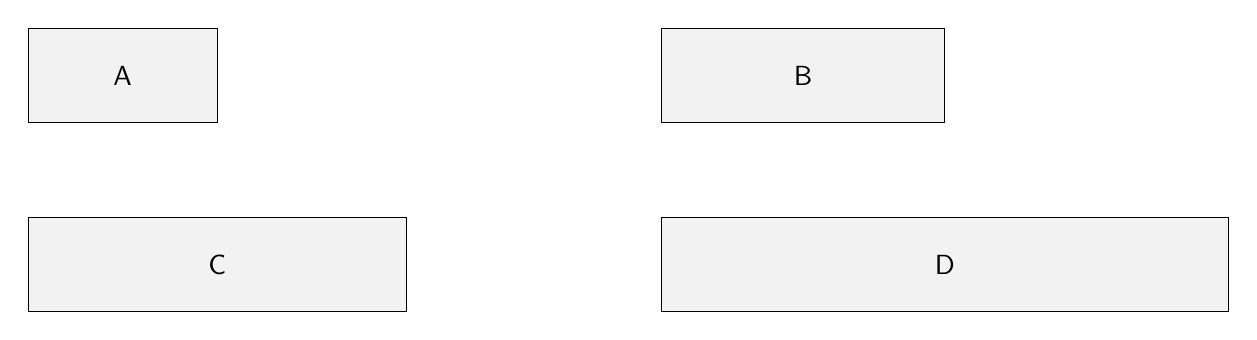
\begin{tikzpicture}[x=12mm,y=12mm]
\foreach \x/\y/\n/\s in {0/0/2/A,6.7/0/3/B,0/-2/4/C,6.7/-2/6/D}{\draw[fill=gray!10] (\x,\y) rectangle +(\n,1);\node at (\x+\n/2,\y+.5){\s};}
\end{tikzpicture}}
\newcommand{\unitrow}{\begin{tikzpicture}[x=12mm,y=12mm]\foreach\i in{0,...,11}{\draw(\i,0) rectangle +(1,1);}\end{tikzpicture}}
\newcommand{\addexample}{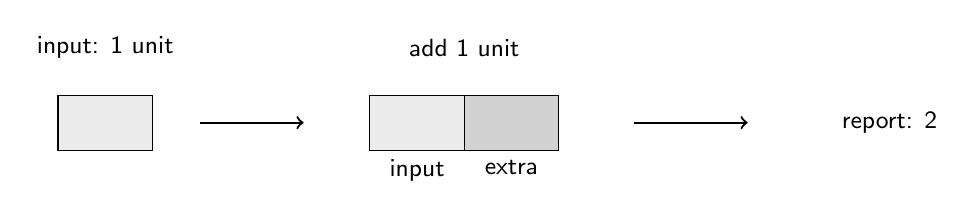
\begin{tikzpicture}[x=12mm,y=10mm,font=\small]
\node at (1.2,1.3){input: 1 unit};\draw[fill=gray!15] (.7,0) rectangle +(1,.7);
\draw[->,thick] (2.2,.35)--(3.3,.35);
\draw[fill=gray!15] (4,0) rectangle +(1,.7);\draw[fill=gray!35] (5,0) rectangle +(1,.7);
\node at (5,1.3){add 1 unit};\node[below] at (4.5,0){input};\node[below] at (5.5,0){extra};
\draw[->,thick] (6.8,.35)--(8,.35);\node at (9.5,.35){report: 2};
\end{tikzpicture}}
\newcommand{\affineexample}{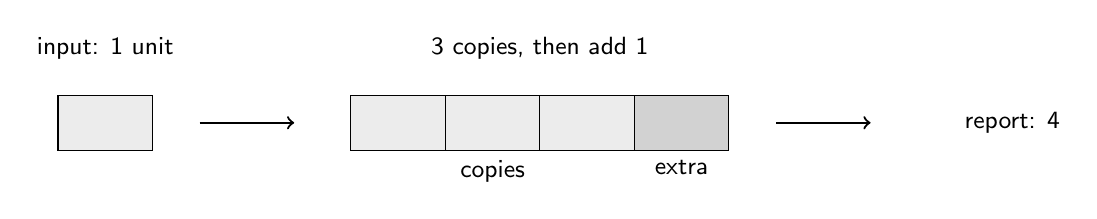
\begin{tikzpicture}[x=12mm,y=10mm,font=\small]
\node at (1,1.3){input: 1 unit};\draw[fill=gray!15] (.5,0) rectangle +(1,.7);
\draw[->,thick](2,.35)--(3,.35);
\foreach\i in{0,...,2}{\draw[fill=gray!15](3.6+\i,0)rectangle+(1,.7);}\draw[fill=gray!35](6.6,0)rectangle+(1,.7);
\node at (5.6,1.3){3 copies, then add 1};\node[below] at(5.1,0){copies};\node[below]at(7.1,0){extra};
\draw[->,thick](8.1,.35)--(9.1,.35);\node at(10.6,.35){report: 4};
\end{tikzpicture}}
\newcommand{\tcubes}[3]{\foreach\j in{1,...,#3}{\draw[fill=gray!15](#1,#2+\j-1)rectangle+(1,1);}}
\newcommand{\tcells}[3]{\foreach\j in{1,...,#3}{\draw[gray!70](#1,#2+\j-1)rectangle+(1,1);}}
\newcommand{\towerexample}{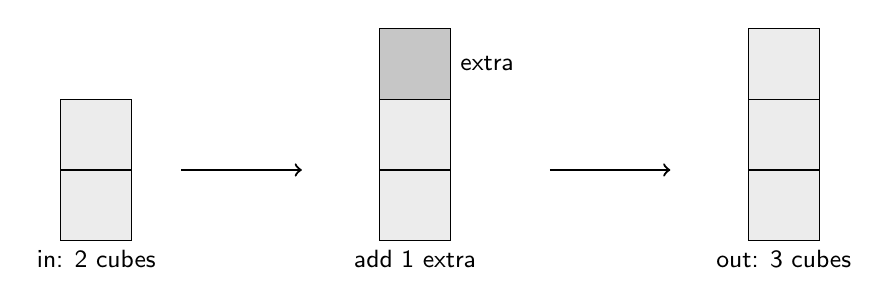
\begin{tikzpicture}[x=9mm,y=9mm,font=\small]
\tcubes{0}{0}{2}\node[below]at(.5,0){in: 2 cubes};
\draw[->,thick](1.7,1)--(3.4,1);
\tcubes{4.5}{0}{2}\draw[fill=gray!45](4.5,2)rectangle+(1,1);\node[right]at(5.5,2.5){extra};
\node[below]at(5,0){add 1 extra};
\draw[->,thick](6.9,1)--(8.6,1);
\tcubes{9.7}{0}{3}\node[below]at(10.2,0){out: 3 cubes};
\end{tikzpicture}}
\begin{document}\fontsize{13}{17}\selectfont
A machine reports a strip's length plus a secret extra number: 1, 2, 3, 4, 5, or 6. The extra number stays the same for the whole round. All lengths are whole units. Each square in the paper row is one unit.
\begin{center}\addexample\end{center}

\problem{1}{Play the machine. Secretly choose an extra number. Your partner gives you a strip; tell them its report. They may ask for more strips until they can name your extra number. Reveal it and switch jobs.}

\begin{center}\begin{tabular}{|p{3.2cm}|p{4.4cm}|p{5.8cm}|}\hline
Round & Strips requested & Reports \\\hline
1\rule{0pt}{10mm}&&\\\hline 2\rule{0pt}{10mm}&&\\\hline 3\rule{0pt}{10mm}&&\\\hline 4\rule{0pt}{10mm}&&\\\hline
\end{tabular}\end{center}
\vspace{3mm}
\begin{center}\unitrow\end{center}
\begin{center}\strips\end{center}

\newpage

\problem{2}{Two hidden strips give these reports. Find every possible pair of lengths.}

\begin{center}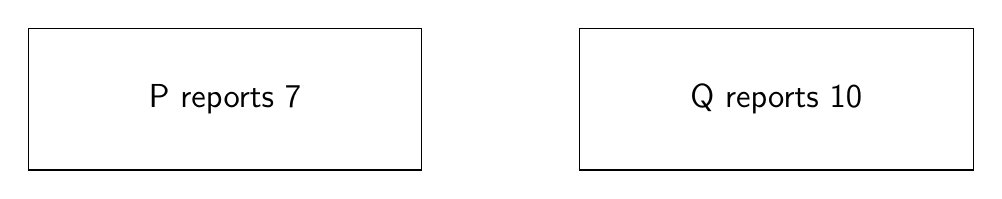
\begin{tikzpicture}[font=\large]
\node[draw,minimum width=5cm,minimum height=1.8cm] at(0,0){P reports 7};
\node[draw,minimum width=5cm,minimum height=1.8cm] at(7,0){Q reports 10};
\end{tikzpicture}\end{center}
\begin{center}\begin{tabular}{|p{4.3cm}|p{4.3cm}|p{4.3cm}|}\hline
Length of P & Length of Q & Extra number \\\hline
\rule{0pt}{15mm}&&\\\hline\rule{0pt}{15mm}&&\\\hline\rule{0pt}{15mm}&&\\\hline\rule{0pt}{15mm}&&\\\hline\rule{0pt}{15mm}&&\\\hline\rule{0pt}{15mm}&&\\\hline\rule{0pt}{15mm}&&\\\hline
\end{tabular}\end{center}

\problem{3}{Could P be longer than Q? What can you know about the two lengths without learning the extra number?}

\room{2cm}

\newpage

\problem{4}{Each row uses a different machine. A known strip gives report 8. Two hidden strips give reports 9 and 12. Build the hidden strips for each row.}

\begin{center}\begin{tabular}{|p{4.8cm}|p{4.1cm}|p{4.1cm}|}\hline
Known strip & Length that reports 9 & Length that reports 12 \\\hline
\rule{0pt}{22mm}4 units $\longrightarrow$ 8&&\\\hline
\rule{0pt}{22mm}6 units $\longrightarrow$ 8&&\\\hline
\rule{0pt}{22mm}2 units $\longrightarrow$ 8&&\\\hline
\end{tabular}\end{center}
\vspace{8mm}

\problem{5}{Your partner knows only that two hidden strips report 7 and 10. Secretly choose a machine and write both hidden lengths under a cover. Let your partner request the report for one known strip, then build each hidden strip. Reveal the lengths and switch jobs.}

\vspace{5mm}
\workbox{5.5}

\newpage

\problem{6}{Each box claims to come from one machine. Which boxes could be right? Repair each impossible box by changing just one report.}

\begin{center}\begin{tabular}{|p{3.7cm}|p{3.7cm}|p{3.7cm}|}\hline
I & II & III \\\hline
2 units $\to$ 5 & 2 units $\to$ 8 & 2 units $\to$ 3 \\
4 units $\to$ 7 & 4 units $\to$ 10 & 4 units $\to$ 6 \\
6 units $\to$ 10 & 6 units $\to$ 12 & 6 units $\to$ 7 \\\hline
\end{tabular}\end{center}
\vspace{6mm}\workbox{4.5}

\problem{7}{Make three length-and-report pairs with exactly one wrong report. Give it to your partner to repair. The correct machine must use one of the six extra numbers.}

\vspace{4mm}\workbox{5.5}
\end{document}
